\chapter{System Design}

%-------------------------------------------------------------------------------------------------------

\section{Requirements Specification}

\subsection{Ability to Plan a Path}
\noindent
The primary functional requirement for this system is the ability to plan a path through a complex environment that can then be traversed by a mobile robot. By a complex environment we refer to a 2D representation stored in some form of map that \textit{may} represent a real world environment. The complexity of the environment is determined by the number of obstacles that the planner must successfully avoid. The success of a journey shall be measured based on the length of the planned path as a percentage when compared to other solutions. \\

\noindent
Given a 2D map, start, and goal position, the planner using \textbf{a path planning algorithm must produce a traversable path}. A path will be made up of a series of points expressed in \textit{x} and \textit{y} coordinates, these can then be iteratively processed. In a case where no path to the goal exists due to obstacles the planning process must be capable of gracefully terminating which includes safely bringing the robot to a halt and providing appropriate feedback. \\

\noindent
\textbf{Inputs:} 2D map, start position, goal position. \\
\textbf{Outputs:} A path of points OR termination feedback.

\newpage

\subsection{Robot Mobility}
\noindent
In order to traverse the path produced as outlined in the previous requirement we need a mobile robot. \textbf{A mobile robot is one that is capable of movement in at least one axis} that will result in a change of position. For our purposes we need to be mobile in both the \textit{x} and \textit{y} axis. The robotic platform's drive system therefore will need to be based on a wheeled, tracked, or legged configuration which can provide the ability to travel on a level surface. It is important to note that the planning system places no restrictions on the dimensions of the robot. \\ 

\noindent
However neither does it account for cases where these dimensions make traversing a path impossible due to space restrictions. The system must be able to make an intelligent decision based on the robot's current position and the next point to travel towards. The output from this requirement is an action that brings us closer towards the goal, this may involve rotating to face the next point along with travelling the calculated distance. \\

\noindent
\textbf{Inputs:} current positon, next postion \\
\textbf{Outputs:} travel distance OR travel distance AND rotate

\subsection{Data Gathering}
\noindent
During the execution of the plannning process the system shall generate a constant stream of data, and a requirement
of this project is to capture this information for later analysis. The type of data being produced can tell us a lot
about the operation including the accuracy, run time, and each planners efficiency. These results must be stored for later analysis in text format. The data attributes that need to be gathered include the planned path, run time, length of the path, and the total number of vertex accesses. \\

\noindent
\textbf{Inputs:} planned path, run time, length of path, total vertex accesses \\
\textbf{Outputs:} time stamped directory containing datasets and plot files

\subsection{Hardware Platform Specification}\label{hardware_specification}
\noindent
As the path planning system implemented on the Linux host is designed to be independent from the hardware specifics of the robot it is necessary that all robots communicate with the planner in a predefined way. We will discuss this mechanism under \ref{sec:protocol} from the software side here we will specify a generic robot that implements the interface. \\

\noindent
In order to be compatible with the planner a robot must have software/hardware:

\begin{itemize}
\item Odometers - capable of establishing an $(x, y)$ position in meters and $\theta$ in radians.
\item Communications - a channel for processing text based data to and from the planner.
\end{itemize}

\noindent
How accurate this hardware needs to be is completely dependent on the application, the planning system can only assume that any data it receives is valid. Any hardware inaccuracies \textit{i.e.} drift must be dealt with at a lower level, the purpose of this approach is to decouple the planner from a robot's implementation details. This enables the planning system to be tested across a wide variety of platforms without having to account for each individual hardware configuration (Figure \ref{Figure: Hardware Agent Specification.}). It is perfectly possible that the planner and robot hardware control be implemented on the same physical system rather than externally this could be done via IP using the \textit{localhost} address.

\begin{figure}[htbp]

\center 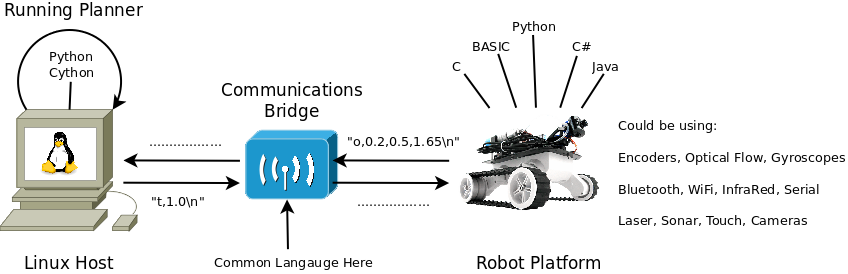
\includegraphics[width=400pt]{illustrations/hardware_agent_specification}\\
\caption{The planner on the Linux host and robot platform communicate via a common communications bridge that they both understand regardless of implementation details.} 
\label{Figure: Hardware Agent Specification.}

\end{figure}

\subsubsection{Motion Model}
\noindent
The planner will impose some restrictions on the motion model that a robot must use to be compatible with the paths it produces. It will be assumed that the robot can perform on the spot rotations, this is necessary as all of the path planning algorithms \textit{may} produce paths that require this kind of motion. In wheeled and tracked vehicles this is typically referred to as \textit{skid steering} \cite{JMD14}, on the spot rotations are achieved by running the drive systems on either side in opposite directions, a tank is good example of this. Legged robots are also capable of performing such turns, however the heading changes can be too extreme for rack-and-pinion based agents \textit{i.e.} cars and trucks. 

\newpage

%-------------------------------------------------------------------------------------------------------

\section{System Modelling}

\subsection{Overview}
\noindent
The navigation system as a whole is built from four key components that when brought together can be used to evaluate the performance of the selected path planning algorithm. These four components are (Figure \ref{overview}):

\begin{enumerate}
\item \textit{Inputs} - operating map and a valid configuration.
\item \textit{System Core} - provides all of the functionality and the interface.
\item \textit{Pluggable Algorithms} - deal specifically with producing paths.
\item \textit{Physical Output} - actual movement of a mobile robot.
\end{enumerate}

\begin{figure}[htbp]

\center 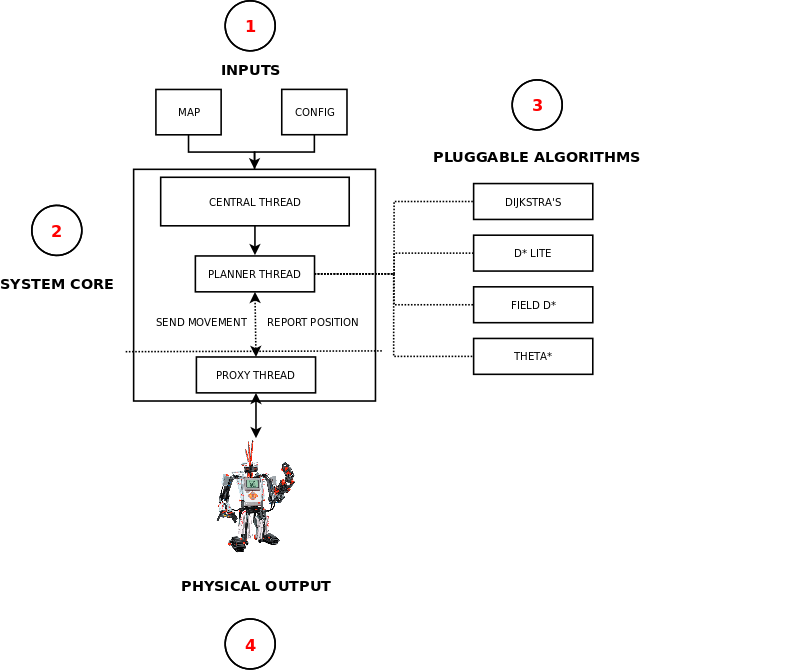
\includegraphics[width=325pt]{illustrations/overview.png}\\
\caption{Individually each component in the system is of limited use but by bringing them together the result is a fully functional path planning system.} 
\label{overview}

\end{figure}

\noindent
In essence the final component \textit{may} not even exist as a physical robot. Instead a computer generated simulation could be used for carrying out large numbers of tests in controlled environments. Each of these components is mutually dependent on the other, we cannot start the system core without both a valid map and configuration, just in the same way without an algorithm there can be no path. This should not be mistaken for \textit{tight coupling}, instead this is a \textit{modular} implementation where each component interacts in an abstract way. When all of these components come together we have a path planning system not just an algorithm.

\subsection{Threaded Architecture}

\noindent
The \textit{BotNav} navigation system contains three separate threads of execution each of which perform a specific task, they are the Central, Proxy, and Planner threads. As threaded programming is notoriously difficult to understand we will cover the architecture here in detail. The task of the three threads can be summarised as follows: 

\begin{itemize}
\item \textbf{Central} - Deals with user input, configuration, initial execution, and pre-emptive termination. 
\item \textbf{Proxy} - Provides a two way communications channel to a physical robot for sending commands and receiving updates.
\item \textbf{Planner} - Interacts with the planning algorithm and produces a string of points that the robot iteratively navigates to.
\end{itemize} 

\subsubsection*{Central Thread}
\noindent
The Central thread deals with user input \textit{i.e.} the configuration file, based on the parameters in the configuration file it \textit{may} spawn both the Proxy \textit{and} Planner threads or just the Planner thread. In simulation mode the Central thread will spawn $n$ Planner threads one after another, where $n$ is the total number of traversable cells, as each Planner finishes another begins. In physical mode only one Planner thread is spawned as it is only practical to carry out one journey with a real robot. \textit{BotNav} terminates execution after all of the Central thread's children finish. Below we can see the basic process flow for the Central thread in Figure \ref{central thread}:

\begin{figure}[htbp]

\center 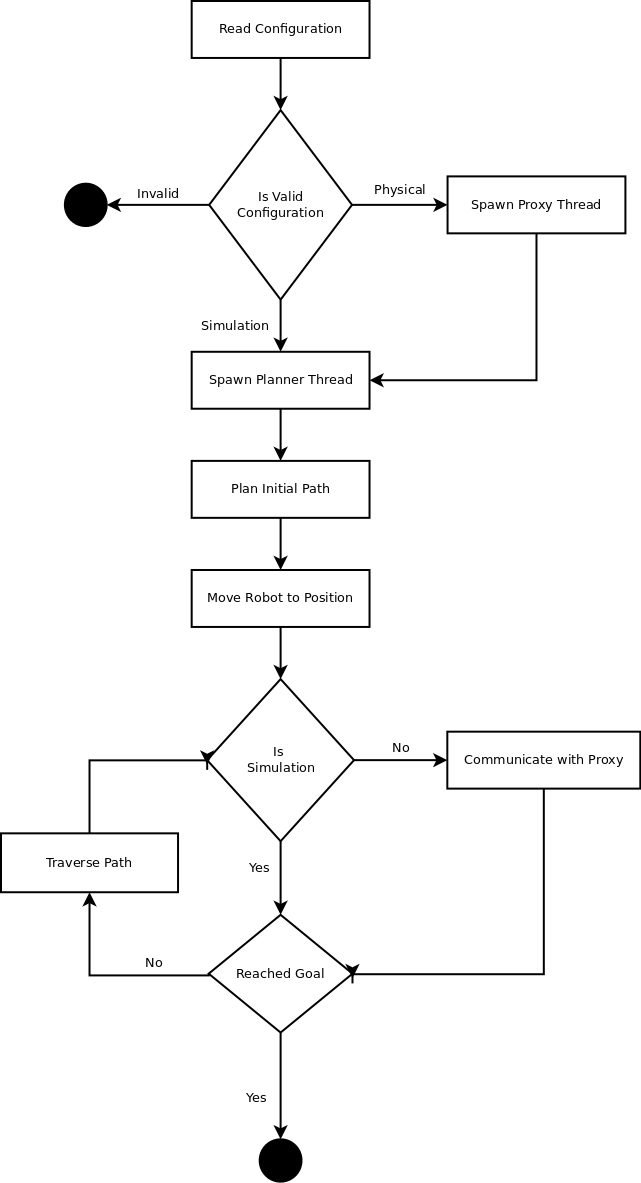
\includegraphics[width=200pt]{illustrations/thread_flow.png}\\
\caption{From reading the configuration file, to deciding upon which child threads to spawn, the Central thread plays a very important part in the execution of the system.} 
\label{central thread}

\end{figure}

\subsubsection*{Proxy Thread}
\noindent
Two way communication with a physical robot that implements the communications protocol outlined in \ref{sec:protocol} is provided via the Proxy thread. The Proxy thread's \textit{passive} function is to process the constant stream of odometry data being generated by the robot, this data is then passed onto the system as odometry updates. 

\subsubsection*{Planner Thread}\label{planner thread}
\noindent
It is in the execution of the Planner Thread where the must crucial work takes place, the Planner brings together a map, robot, proxy, and planning algorithm. All of this is achieved in such a way that it is possible to plug any one of the planning algorithms implemented for this project (GridNav, D* Lite, Field D*, Theta*) into it. \\

\noindent
During a planning cycle the Planner Thread calls upon the planning algorithms \textit{plan} routine which uses a combination of the robot's current position, a goal, and an occupancy grid to produce a path. The actual implementation behind a particular algorithm's planning functionality is hidden from the Planner Thread. If there is a valid path the result of the call to \textit{plan} will be a trail of points which the robot can then iteratively traverse. In the case where no path exists to the goal execution is immediately terminated. \\

\noindent
Once a path has been generated and returned it is processed as follows: \\

\begin{lstlisting}
while we are not within 0.7 cells of the goal in both x and y:
	# Scan the immediate area.
	robot.scan()
	
	# Check for a change in the map.
	if there is a change:
		path = algorithm.plan()
		
	# Pop the next point from the current path.
	if path length is 0:  # Make sure there is a point.
		break

	point = path.pop() # Get the next point.
	robot.go(point.x, point.y)
	
	while robot is travelling:
		# Busy wait.

	calculate x difference to goal
	calculate y difference to goal
\end{lstlisting}

%-------------------------------------------------------------------------------------------------------

\section{Communications Protocol}\label{sec:protocol}
\noindent
This section briefly discusses the communications protocol that a physical hardware robot must implement in order to be compatible with the planning system. The protocol covered here is an extension of the simple communications mechanism from \cite{JMD14} that was used to drive a tele-operated mapping robot. It is based on plain text strings terminated by new line characters (`$\backslash$n') and was designed with simplicity in mind. All commands are synchronous in behaviour and cannot be completed until the appropriate response has been returned. The full specification is available in the Appendices under section \ref{Appendix: Communications Protocol Specification}.

\subsection{Travelling a Predefined Distance}
\noindent
To instruct the robot to travel forward for a straight line distance of 1.3 metres the command is simply: \\

\textit{t,1.3$\backslash$n} \\

\noindent
The `t' character literally stands for \textit{``travel"}, the distance specified as a decimal number comes immediately after the `,' character and can be any \textbf{positive} value, it must be terminated by a newline character. When the robot has completed the command it simply responses with the string: \\

\textit{Travelled$\backslash$n} \\

\noindent
This informs the planner that the robot is no longer in motion and that the next planning step can now be processed. It is possible for a robot's local planner or obstacle avoidance system to abort the action by simply returning this response at any stage in the journey due to unforeseen obstacles. In these cases the robot should return the location of the obstacle(s) in its next scan report.

\subsection{Rotating to a Given Heading}
\noindent
Valid headings run from $0-6.27 rads$ in a circular fashion, they increase from right to left around the circle. To instruct the robot to face a heading of 1.57 radians ($90^{\circ}$) the command is: \\

\textit{r,1.57$\backslash$n} \\

\noindent
There is no explicit return value instead the planner waits until the odometry reports from the robot are within 0.02 radians ($1^{\circ}$) of the requested heading, the robot is then instructed to stop if it has not already done so. The planner uses both the travel and rotation commands in conjunction to navigate to specific points. \\

\noindent
First the robot is commanded to face a given point then the distance between its position and the target are calculated, secondly the robot is sent a travel command containing this information. Using this mechanism the robot is able to navigate complex environments with only the basic knowledge it requires, the rest is done by the planner.

%-------------------------------------------------------------------------------------------------------

\section{Programming Platforms}

\subsection{Linux Architecture}
\noindent
The Linux kernel is to date driving an increasing number of commercial and research robotic platforms all over the world including Google's Self Car Project, Nao, EV3 Lego Mindstorms, and the horde of robots that use ROS \cite{MIT, NAO, EV3, ROS}. Linux is stable, customisable, embeddable, and freely available, making it a suitable candidate for powering robotic systems. \\

\begin{figure}[htbp]

\center 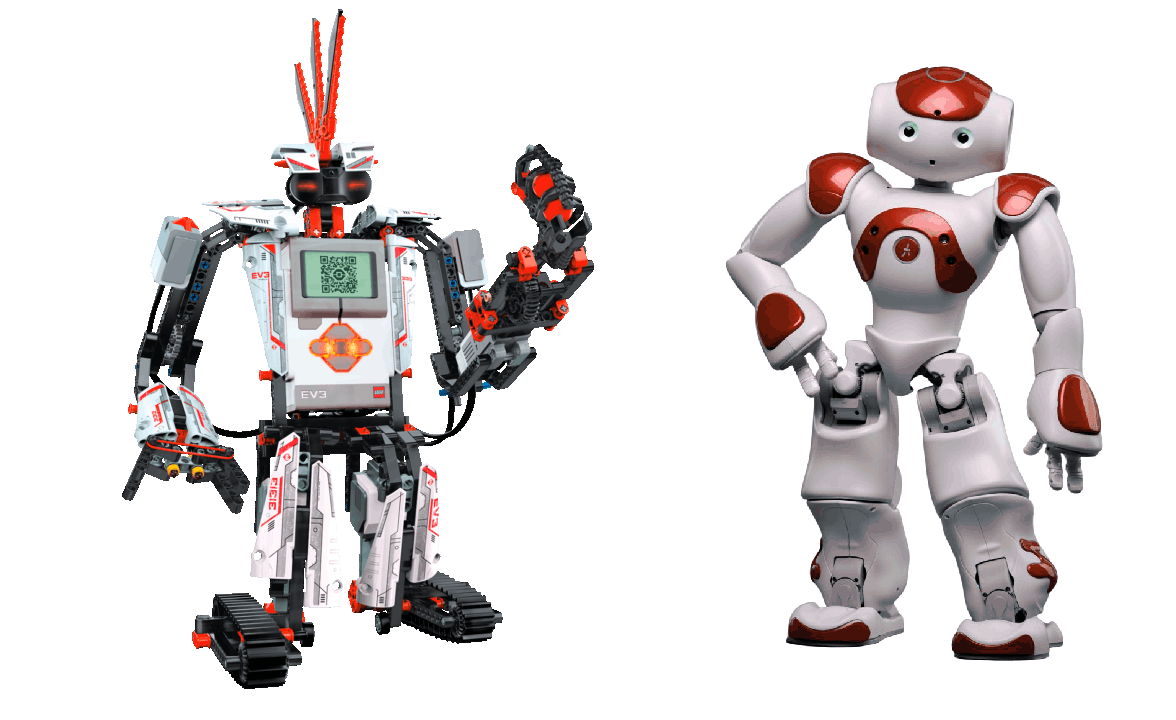
\includegraphics[width=300pt]{illustrations/ev3_nao.png}\\
\caption{Both the EV3 Lego Mindstorms (left) and the Nao (right) run a distribution of the Linux Kernel. \cite{EV3, NAO}} 
\label{central thread}

\end{figure}

\noindent
Considering all of the points previously mentioned Linux was picked as the target programming platform over any other alternatives. Linux's embeddable nature is important to this project as at least one of the physical robots may be equipped with the \textit{Raspberry Pi} a credit card size computer capable of running Linux. The system will be tested on two distributions of Linux, one embedded on the robot(s), the other connected externally:

\begin{itemize}
\item Raspbian (Embedded)
\item Ubuntu Linux 14.10 (External)
\end{itemize} 

\newpage

\subsection{Python3}
Python version 3 (Python3) has been selected as the most appropriate core programming language for the implementation stage for the following reasons:

\begin{itemize}
\item Development Speed - Python is an interpreted bytecode language which is compiled ``on the fly" eliminating lengthy build overheads.
\item Interactive Shell - Python's shell facilitates interactive programming which lends itself to test driven coding.
\item Python and Robotics - already widely used in the robotics field, Sebastian Thurn's Udacity program is done purely using Python \cite{THRUN}.
\end{itemize} 

\noindent
Python's syntax is also extremely lenient when compared to compiled languages such as C where every variable must explicitly declare its type before it can be used, making the equivalent Python code more visually compact. The implementation could have been carried out using C, C++, Java, or C$\sharp$ as the author already has experience in those languages, however using Python instead presents a unique learning opportunity. 

\subsection{Cython Modules}
\noindent
A major drawback of interpreted languages is the speed of their execution when compared to compiled languages, since Python is implemented using a virtual machine it will nearly always be slower than pure machine code. It is important to take this issue into account at design time as the planning algorithms are computationally complex and as the state space increases Python will become less adapt at handling it compared to a compiled language. \\

\noindent
Fortunately as Python is wrote in C it can also be extended using C. Implementing the planning algorithms as Cython modules shall significantly increase their performance while still enabling the rest of the system to use Python. At the time of writing GCC (GNU C Compiler) version 4.9.1 has been selected for compilation purposes.

%-------------------------------------------------------------------------------------------------------

\newpage

\section{Source Control}
This section covers how the project was managed, the source control system used, frequency off commits, total commits, and any branching.

\subsection{Git}
\noindent
Throughout the projects development all work undertaken including everything from the code base, poster, modelling, and thesis was managed and controlled using the Git source control tool. This decision was taken at design time as it came with a number of distinct advantages such as providing a clear work history and the ability to roll back changes if the need arose. Another important reason for choosing Git over other systems is that it maintains a local copy in addition to the working head in the remote repository \cite{GIT}. An open repository was set-up and maintained in the cloud at the GitHub \href{https://www.github.com/swordmaster2k/botnav}{\textit{BotNav}}.

\newpage

%-------------------------------------------------------------------------------------------------------
